\documentclass[tikz,border=5pt]{standalone}
\usetikzlibrary{calc}
\begin{document}

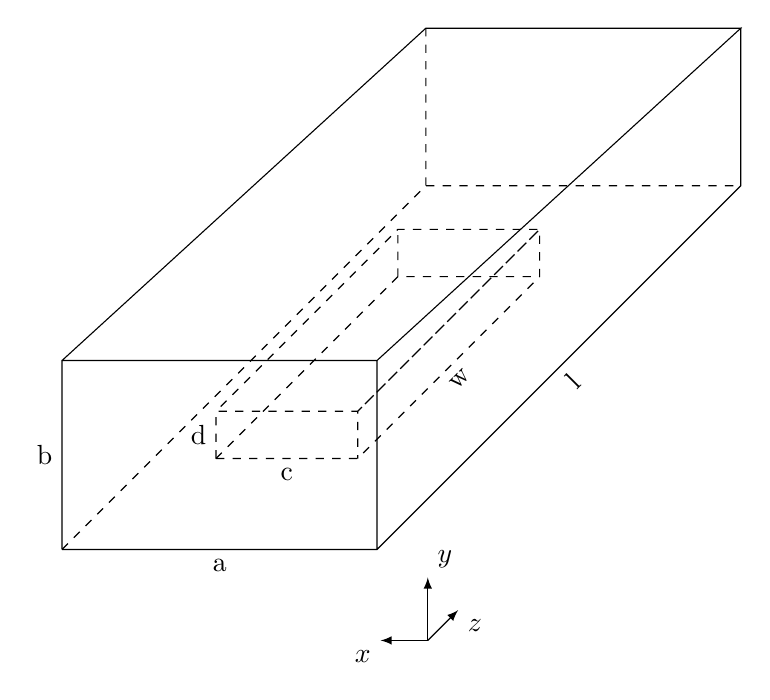
\begin{tikzpicture}[>=latex,scale=2]
\pgfmathsetmacro{\x}{2.0}
\pgfmathsetmacro{\xb}{1.7}
\pgfmathsetmacro{\y}{6.0}
\pgfmathsetmacro{\z}{1.2}
\pgfmathsetmacro{\zb}{1.0}

\path (0,0,\y) coordinate (A) (\x,0,\y) coordinate (B) (\x,0,0) coordinate (C) (0,0,0)
coordinate (D) (0,\z,\y) coordinate (E) (\x,\z,\y) coordinate (F) (\x,\zb,0) coordinate (G)
(0,\zb,0) coordinate (H);
\draw (A)-- node[below]{a} (B)-- node[below,sloped]{l} (C)--(G)--(F)--(B) (A)-- node[left]{b}(E)--(F)--(G)--(H)--(E);
\draw [dashed,black] (A)--(D)--(C) (D)--(H);

\pgfmathsetmacro{\xdelta}{0.4}
\pgfmathsetmacro{\ydelta}{1.5}
%\pgfmathsetmacro{\zdelta}{0.4}
\pgfmathsetmacro{\xprime}{1.3}
\pgfmathsetmacro{\xbprime}{1.2}
\pgfmathsetmacro{\yprime}{4.5}
\pgfmathsetmacro{\zprime}{0.3}

\path (\xdelta,0,\yprime) coordinate (Ap) (\xprime,0,\yprime) coordinate (Bp) (\xprime,0,\ydelta) coordinate (Cp) (\xdelta,0,\ydelta)
coordinate (Dp) (\xdelta,\zprime,\yprime) coordinate (Ep) (\xprime,\zprime,\yprime) coordinate (Fp) (\xprime,\zprime,\ydelta) coordinate (Gp)
(\xdelta,\zprime,\ydelta) coordinate (Hp);

\draw [dashed,black] (Ap)-- node[below]{c} (Bp)-- node[below,sloped]{w} (Cp)--(Gp)--(Fp)--(Bp) (Ap)-- node[left]{d}(Ep)--(Fp)--(Gp)--(Hp)--(Ep);
\draw [dashed,black] (Ap)--(Dp)--(Cp) (Dp)--(Hp);

\draw[->](2.9,0,7.5)--(2.9,0,7.0)node[anchor=north west]{$z$};
\draw[->](2.9,0,7.5)--(2.6,0,7.5)node[anchor=north east]{$x$};
\draw[->](2.9,0,7.5)--(2.9,0.4,7.5)node[anchor=south west]{$y$};

\end{tikzpicture}

\end{document}
